\section{C1. Description de l’architecture mise en place}

\textcolor{red}{Pour le 05/01/2016.} \\

\textcolor{red}{C1. Description de l’architecture mise en place pour réaliser une expérience permettant sur la solution technique X de mesurer les indicateurs contribuant à la comparaison. Par description de l’architecture est entendu un diagramme de déploiement (au sens UML) faisant apparaître le(s) noeud(s) matériel(s), les composants ainsi que les artefacts utilisés par les composants. On veillera à ce que les composants présentés aient, dans leur ensemble, une granularité cohérente.}\\

	\begin{figure}[h!]
		\centering
		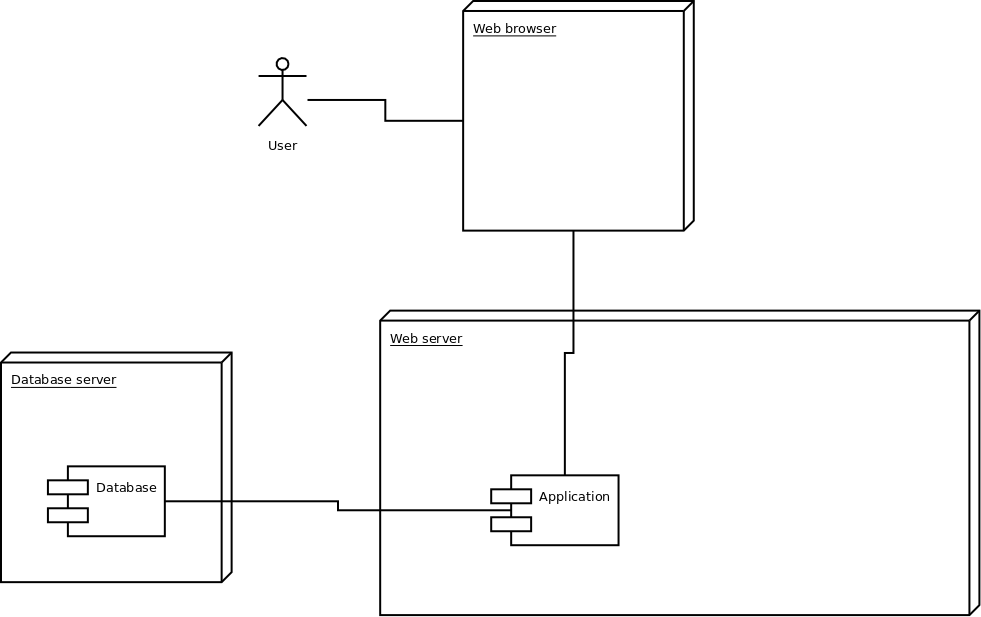
\includegraphics[width=18cm]{./images/diagDep.png}
		\caption{Diagramme de déploiement}
	\end{figure}
